\documentclass[14pt]{extbook}
\usepackage{multicol, enumerate, enumitem, hyperref, color, soul, setspace, parskip, fancyhdr} %General Packages
\usepackage{amssymb, amsthm, amsmath, bbm, latexsym, units, mathtools} %Math Packages
\everymath{\displaystyle} %All math in Display Style
% Packages with additional options
\usepackage[headsep=0.5cm,headheight=12pt, left=1 in,right= 1 in,top= 1 in,bottom= 1 in]{geometry}
\usepackage[usenames,dvipsnames]{xcolor}
\usepackage{dashrule}  % Package to use the command below to create lines between items
\newcommand{\litem}[1]{\item#1\hspace*{-1cm}\rule{\textwidth}{0.4pt}}
\pagestyle{fancy}
\lhead{Progress Quiz 1}
\chead{}
\rhead{Version A}
\lfoot{1269-8776}
\cfoot{}
\rfoot{Fall 2020}
\begin{document}

\begin{enumerate}
\litem{
Write the equation of the line in the graph below in Standard form $Ax+By=C$. Then, choose the intervals that contain $A, B, \text{ and } C$.
\begin{center}
    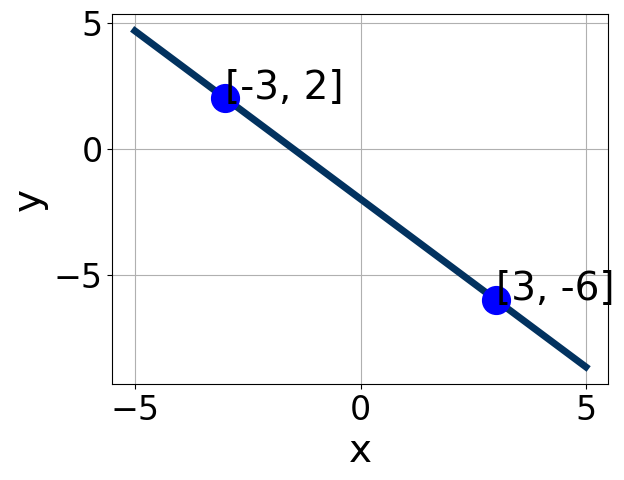
\includegraphics[width=0.5\textwidth]{../Figures/linearGraphToStandardA.png}
\end{center}
\begin{enumerate}[label=\Alph*.]
\item \( A \in [-9, 0], \hspace{3mm} B \in [-5.4, -3.2], \text{ and } \hspace{3mm} C \in [-15, -7] \)
\item \( A \in [4, 5], \hspace{3mm} B \in [1.4, 8.3], \text{ and } \hspace{3mm} C \in [9, 13] \)
\item \( A \in [-0.2, 1.8], \hspace{3mm} B \in [-4.4, 0.8], \text{ and } \hspace{3mm} C \in [-6, 0] \)
\item \( A \in [-0.2, 1.8], \hspace{3mm} B \in [0.7, 2.1], \text{ and } \hspace{3mm} C \in [1, 3] \)
\item \( A \in [4, 5], \hspace{3mm} B \in [-5.4, -3.2], \text{ and } \hspace{3mm} C \in [-15, -7] \)

\end{enumerate} }
\litem{
Find the equation of the line described below. Write the linear equation as $ y=mx+b $ and choose the intervals that contain $m$ and $b$.\[ \text{Perpendicular to } 6 x - 7 y = 12 \text{ and passing through the point } (-6, 9). \]\begin{enumerate}[label=\Alph*.]
\item \( m \in [-1.32, -1.04] \hspace*{3mm} b \in [-2.34, -1.24] \)
\item \( m \in [-1.32, -1.04] \hspace*{3mm} b \in [1.63, 2.84] \)
\item \( m \in [-1.32, -1.04] \hspace*{3mm} b \in [14.04, 15.25] \)
\item \( m \in [-1, -0.63] \hspace*{3mm} b \in [1.63, 2.84] \)
\item \( m \in [0.65, 1.44] \hspace*{3mm} b \in [15.67, 16.48] \)

\end{enumerate} }
\litem{
First, find the equation of the line containing the two points below. Then, write the equation as $ y=mx+b $ and choose the intervals that contain $m$ and $b$.\[ (4, 10) \text{ and } (-9, -2) \]\begin{enumerate}[label=\Alph*.]
\item \( m \in [-2.4, -0.29] \hspace*{3mm} b \in [-10.39, -9.79] \)
\item \( m \in [0.31, 1.9] \hspace*{3mm} b \in [5.78, 6.11] \)
\item \( m \in [0.31, 1.9] \hspace*{3mm} b \in [6.61, 7.18] \)
\item \( m \in [0.31, 1.9] \hspace*{3mm} b \in [6.15, 6.33] \)
\item \( m \in [0.31, 1.9] \hspace*{3mm} b \in [-6.81, -6.26] \)

\end{enumerate} }
\litem{
Solve the equation below. Then, choose the interval that contains the solution.\[ -11(-8x + 9) = -6(-12x -18) \]\begin{enumerate}[label=\Alph*.]
\item \( x \in [-0.2, -0.09] \)
\item \( x \in [-7.6, -7.2] \)
\item \( x \in [0.75, 1.29] \)
\item \( x \in [-0.82, -0.56] \)
\item \( \text{There are no real solutions.} \)

\end{enumerate} }

\litem{
Solve the linear equation below. Then, choose the interval that contains the solution.\[ \frac{-8x + 9}{3} - \frac{-6x + 9}{5} = \frac{-9x -9}{8} \]\begin{enumerate}[label=\Alph*.]
\item \( x \in [4.8, 10.8] \)
\item \( x \in [-2.33, 4.67] \)
\item \( x \in [17.34, 23.34] \)
\item \( x \in [23.34, 29.34] \)
\item \( \text{There are no real solutions.} \)

\end{enumerate} }
\litem{
Write the equation of the line in the graph below in Standard form $Ax+By=C$. Then, choose the intervals that contain $A, B, \text{ and } C$.
\begin{center}
    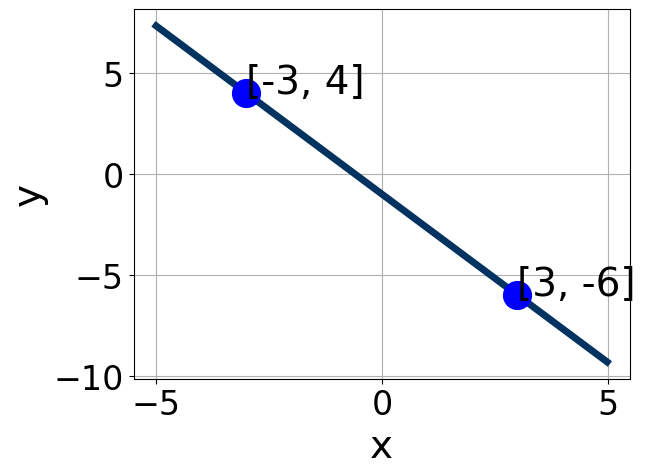
\includegraphics[width=0.5\textwidth]{../Figures/linearGraphToStandardCopyA.png}
\end{center}
\begin{enumerate}[label=\Alph*.]
\item \( A \in [0.5, 1.4], \hspace{3mm} B \in [0.64, 1.2], \text{ and } \hspace{3mm} C \in [1, 14] \)
\item \( A \in [0.5, 1.4], \hspace{3mm} B \in [-1.53, -0.68], \text{ and } \hspace{3mm} C \in [-5, 3] \)
\item \( A \in [3.2, 5.7], \hspace{3mm} B \in [3.92, 4.65], \text{ and } \hspace{3mm} C \in [12, 18] \)
\item \( A \in [-5.1, -1.3], \hspace{3mm} B \in [-4.91, -3.42], \text{ and } \hspace{3mm} C \in [-16, -12] \)
\item \( A \in [3.2, 5.7], \hspace{3mm} B \in [-4.91, -3.42], \text{ and } \hspace{3mm} C \in [-16, -12] \)

\end{enumerate} }
\litem{
Find the equation of the line described below. Write the linear equation as $ y=mx+b $ and choose the intervals that contain $m$ and $b$.\[ \text{Perpendicular to } 9 x + 4 y = 14 \text{ and passing through the point } (9, 5). \]\begin{enumerate}[label=\Alph*.]
\item \( m \in [0.19, 1.41] \hspace*{3mm} b \in [-5.5, -2.8] \)
\item \( m \in [0.19, 1.41] \hspace*{3mm} b \in [-0.1, 1.5] \)
\item \( m \in [0.19, 1.41] \hspace*{3mm} b \in [-2.8, 0.3] \)
\item \( m \in [-1.39, 0.09] \hspace*{3mm} b \in [7.4, 9.5] \)
\item \( m \in [1.21, 2.78] \hspace*{3mm} b \in [-0.1, 1.5] \)

\end{enumerate} }
\litem{
First, find the equation of the line containing the two points below. Then, write the equation as $ y=mx+b $ and choose the intervals that contain $m$ and $b$.\[ (-3, -7) \text{ and } (4, 4) \]\begin{enumerate}[label=\Alph*.]
\item \( m \in [1.57, 4.57] \hspace*{3mm} b \in [-2.1, 0.1] \)
\item \( m \in [1.57, 4.57] \hspace*{3mm} b \in [-2.4, -1.7] \)
\item \( m \in [1.57, 4.57] \hspace*{3mm} b \in [0.6, 2.6] \)
\item \( m \in [1.57, 4.57] \hspace*{3mm} b \in [-6, -3.8] \)
\item \( m \in [-5.57, 1.43] \hspace*{3mm} b \in [8.9, 11.9] \)

\end{enumerate} }

\litem{
Solve the equation below. Then, choose the interval that contains the solution.\[ -12(10x + 5) = -3(19x -14) \]\begin{enumerate}[label=\Alph*.]
\item \( x \in [-54.4, -52] \)
\item \( x \in [-26.7, -24.5] \)
\item \( x \in [0.6, 2.3] \)
\item \( x \in [-3.1, -1.3] \)
\item \( \text{There are no real solutions.} \)

\end{enumerate} }

\litem{
Solve the linear equation below. Then, choose the interval that contains the solution.\[ \frac{-3x + 3}{5} - \frac{9x + 5}{8} = \frac{-8x -5}{6} \]\begin{enumerate}[label=\Alph*.]
\item \( x \in [3.7, 6.1] \)
\item \( x \in [-0.9, 1] \)
\item \( x \in [6.8, 8.4] \)
\item \( x \in [1, 2.9] \)
\item \( \text{There are no real solutions.} \)

\end{enumerate} }
\end{enumerate}

\end{document}